\documentclass{report}
\begin{document}
\chapter{Pendahuluan}
\section{Latar Belakang}
\par Sistem keamanan Jaringan merupakan hal yang sangat penting untuk dikembangkan untuk menjaga kerahasiaan dan keamanan data. Karena data merupakan hal yang sangat vital dalam kehidupan di zaman modern ini.
\par
Akan tetapi seiring dengan perkembangan teknologi, semakin banyaknya \textit{software} yang dikembangkan, sehingga banyak pula celah keamanan yang timbul. Sehingga, kebutuhan dalam teknologi keamanan jaringan menjadi sangat banyak pula.
\subsection{Data terkait}
Dilansir dari \textit{Kaspersky Securelist} persebaran virus terbesar dari periode pelaporan Trojan-Banker.AndroidOS.Asacub. Ini memuncak pada bulan September ketika lebih dari 250.000 pengguna diserang - dan semua itu hanya mencakup statistik bagi mereka yang memiliki produk seluler Kaspersky Lab yang diinstal pada perangkat mereka.\par
\makebox{
\centering
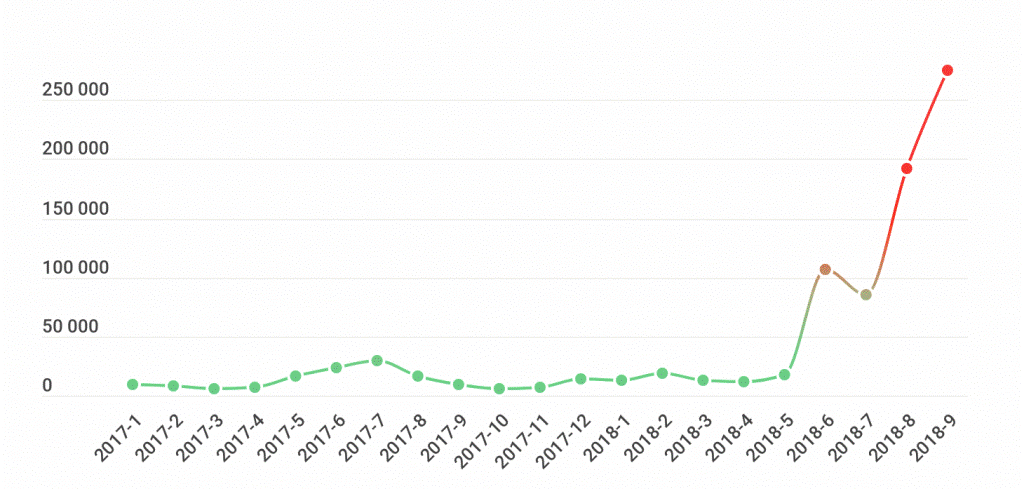
\includegraphics[width=\textwidth]{skripsi/1statistik}
}
\captionof{figure}{Jumlah pengguna yang diserang oleh mobile banker Asacub pada tahun 2017 dan 2018}\label{1statistik}
\cite{chebysev_sinitsyn_parinov_kupreev_lopatin_liskin}
\par
Dari data diatas dapat diamati bahwa penyebaran virus jenis Trojan-Banker ini selalu meningkat.
\subsection{Penelitian terkait}
\section{Rumusan Masalah}
Dari latar belakang dapat dirumuskan masalah sebagai berikut:
\begin{enumerate}
    \item Bagaimana karakteristik intrusi \textit{Binary Virus} yang dapat dideteksi dan tidak dapat dideteksi oleh IDS ?
    \item Bagaimana proses pemodelan \textit{Recurrent Neural Network} untuk mendeteksi intrusi \textit{Binary Virus} pada jaringan ?
    \item Bagaimana proses optimasi \textit{Recurrent Neural Network} untuk memprediksi intrusi \textit{Binary Virus} pada jaringan ?
    \item Bagaimana hasil prediksi pemodelan \textit{Recurrent Neural Network} untuk memprediksi intrusi \textit{Binary Virus} pada jaringan ?
\end{enumerate}
\section{Batasan Masalah}
\begin{enumerate}
    \item Jenis malware yang di analisis merupakan malware berjenis \textit{Binary Virus} dengan metode pendeteksian \textit{signature}
    \item RNN digunakan untuk memprediksi kecenderungan intrusi
    \item IDS diuji tanpa mengaktifkan rule dari \textit{preprocessor} lain
    \item IDS di implementasikan pada jaringan lokal (LAN)
\end{enumerate}
\section{Tujuan}
\begin{enumerate}
    \item Mengintegrasikan kecerdasan buatan dalam penerapannya di bidang keamanan jaringan
    \item Meningkatkan kapabilitas sistem keamanan jaringan untuk pendeteksian intrusi dengan metode RNN
    \item Mengukur kemampuan RNN dalam melakukan pendeteksian dan penyaringan data pada IDS
    \item Mengoptimalkan efektifitas kinerja RNN dalam pendeteksian virus dan otomasi rule pada IDS
\end{enumerate}
\section{Manfaat}
\begin{enumerate}
    \item Memberikan kemudahan dalam pendeteksian intrusi \textit{Binary Virus}
    \item Menjadi referensi untuk mengimplementasikan sistem RNN pada IDS
    \item Menjadi solusi untuk kegiatan pencarian pola untuk dijadikan rule atau tidak
\end{enumerate}
\section{Sistematika Penulisan}
Untuk mencapai tujuan yang diharapkan, maka sistematika penulisan yang disusun dalam tugas akhir ini dibagi menjadi 5 bab sebagai berikut :
\begin{itemize}
    \item Bab I. Pendahuluan \\ Bab ini membahas tentang latar belakang, rumusan masalah, batasan masalah, tujuan penelitian, manfaat penelitian, dan sistematika penulisan
    \item Bab II. Tinjauan Pustaka dan Landasan Teori \\ Bab ini memuat tentang tinjauan pustaka yang menjabarkan hasil penelitian yang berkaitan dengan penelitian ini dan landasan teori yang menjabarkan teori-teori penunjang yang berhubungan dengan penelitian ini.
    \item Bab III. Metedologi Penelitian \\ Memuat tentang metode penelitian, mulai dari pelaksanaan penelitian, diagram alir penelitian, menentukan alat dan bahan, lokasi penelitian, dan langkah-langkah penelitian.
    \item Bab IV. Hasil Penelitian
    \item Bab V. Penutup
\end{itemize}
\end{document}